% Figure 1
\ffigbox[\FBwidth]{
\caption{\centering Cas cycle pair}\label{Fig:td1ex3c2}
}{
    \fbox{
        \resizebox{!}{3cm}{%
            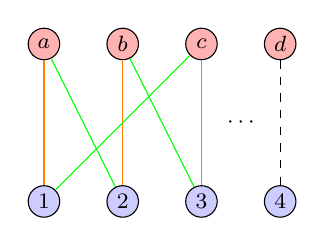
\begin{tikzpicture}[scale=1, every node/.style={circle, draw, fill=blue!20, inner sep=1pt, font=\footnotesize, minimum size=4mm}]
                \node[fill=red!30] (a) at (0, 2) {\(a\)};
                \node[fill=red!30] (b) at (1, 2) {\(b\)};
                \node[fill=red!30] (c) at (2, 2) {\(c\)};
                \node[fill=red!30] (d) at (3, 2) {\(d\)};

                \node (1) at (0, 0) {\(1\)};
                \node (2) at (1, 0) {\(2\)};
                \node (3) at (2, 0) {\(3\)};
                \node (4) at (3, 0) {\(4\)};

                \node[draw=none, fill=none] (dots) at (2.5, 1) {\(\cdots\)};

                \draw[orange] (a) -- (1);
                \draw[orange] (b) -- (2);
                \draw[orange] (c) -- (3);

                \draw[green] (1) -- (c);
                \draw[green] (2) -- (a);
                \draw[green] (3) -- (b);
                
                \draw[dashed] (d) -- (4);
            \end{tikzpicture}
        }
    }
}